\chapter{从线性磁岛到Rutherford增长与薄片破碎}\label{tm:nonlinear}
\section{什么时候线性化失效：比较两个实际项}
线性化删掉了$[\phi_1,\psi_1]$。在常磁通近似下，
\begin{equation}
 \psi\simeq \frac{B'_0x^2}{2}+\widetilde\psi(t)\cos(ky).
\end{equation}
磁通方程中的两个平流贡献分别具有量级
\begin{equation}
 |[\phi_1,\psi_0]|\sim k\phi_1 B'_0\delta,\qquad
 |[\phi_1,\psi_1]|\sim \frac{\phi_1}{\delta}\,k\widetilde\psi.
\end{equation}
二者比值为
\begin{equation}
 \frac{|[\phi_1,\psi_1]|}{|[\phi_1,\psi_0]|}
 \sim\frac{\widetilde\psi}{B'_0\delta^2}
 =\frac{W^2}{16\delta^2}.
 \label{tm:nonlinratio}
\end{equation}
所以线性阶段要求岛宽远小于内层尺度，$W\ll\delta$为常用量级表述；当$W$与$\delta$同量级时，已不能忽略非线性。式中的16来自我们对全宽的定义，而实际内层尺度本身也有定义差别，因此不应把$W=4\delta$当成精确普适的开关。\citep{TMFitzIsland}

此时并不意味着立刻发生爆发性快重联。经典弱驱动、常磁通磁岛往往先进入更慢的Rutherford阶段；大$\Delta'$、强流剪切、双流体或多岛相互作用则可采用不同路径。

\section{Rutherford阶段增加了什么排序}
取
\begin{equation}
 \delta_{\rm linear}\ll W\ll a,\qquad \Delta'W\ll1.
 \label{tm:Rutherfordordering}
\end{equation}
第一个不等式说磁岛已经超过线性层，第二个说岛相对平衡仍小，第三个说岛内扰动电流仍是平衡电流的小修正。模演化慢到惯性可在主阶磁岛平衡中忽略。因此涡量方程给
\begin{equation}
 [\psi,J_z]\simeq0.
\end{equation}
沿磁场的导数为$[\psi,J_z]$，所以它意味着电流在同一磁通面上近似不变：
\begin{equation}
 J_z=J_z(\psi,t).
\end{equation}
这是磁力平衡的限制，不是随意假设电流在整个空间均匀。不同磁通面仍可有不同电流。\citep{TMRutherford1973,TMFitzRutherford}

在岛宽比平衡尺度小的区域，平衡电流近似为常数$J_0=B'_0/\mu_0$。记其小修正为$j(\psi,t)$。扣除背景缓慢扩散或维持平衡的外源后，局地磁通方程为
\begin{equation}
 \dot{\widetilde\psi}\cos\theta+[\phi,\psi]=\eta j(\psi,t),
 \qquad \theta=ky.
 \label{tm:RutherfordOhm}
\end{equation}
点上的平流仍然存在。接下来消去它需要沿闭合磁面的平均，而不是直接宣布$[\phi,\psi]=0$。

\section{磁面平均：为什么能消掉平流项}
用全宽$W=4\sqrt{\widetilde\psi/B'_0}$定义
\begin{equation}
 X=\frac{4x}{W},\qquad
 \Omega=\frac{\psi}{\widetilde\psi}=\frac{X^2}{2}+\cos\theta.
\end{equation}
$\Omega=-1$为O点，$\Omega=1$为分离线，$-1<\Omega<1$在岛内，$\Omega>1$在岛外。给定磁面上
\begin{equation}
 X=\pm\sqrt{2(\Omega-\cos\theta)}.
\end{equation}
设$\mathcal A_\Omega$为该磁面允许的角度集合：岛外为$[0,2\pi]$；岛内为$[\arccos\Omega,\,2\pi-\arccos\Omega]$。对两侧对称的量，定义一个未归一化加权平均
\begin{equation}
 \langle A\rangle_\Omega
 =\frac1{2\pi}\int_{\mathcal A_\Omega}
 \frac{A(\Omega,\theta)}{\sqrt{2(\Omega-\cos\theta)}}\,\dd\theta.
 \label{tm:fluxavg}
\end{equation}
真正的磁面均值是$\langle A\rangle_\Omega/\langle1\rangle_\Omega$。分母不能忘掉；它反映沿磁面不同位置的权重。

为什么恰好用这个权重？在固定$\psi$、亦即固定$\Omega$的磁面上，
\begin{equation}
 [\phi,\psi]
 =-\psi_x\left.\frac{\partial\phi}{\partial y}\right|_\psi
 =-kB'_0x\left.\frac{\partial\phi}{\partial\theta}\right|_\Omega.
\end{equation}
其中第一步可由固定$\psi$时$\dd x/\dd y=-\psi_y/\psi_x$和链式法则直接验证。把它除以$|x|$再沿两侧闭合轨道积分，就是同一单值流函数$\phi$的总变化；闭合一周为零。式\eqref{tm:fluxavg}的权重正比$1/|x|$。因此对式\eqref{tm:RutherfordOhm}进行该平均，平流项被消去：
\begin{equation}
 \boxed{
 j(\Omega,t)=\frac{\dot{\widetilde\psi}}{\eta}
 \frac{\langle\cos\theta\rangle_\Omega}{\langle1\rangle_\Omega}.}
 \label{tm:Rutherfordj}
\end{equation}
这一步把电流修正与磁通幅的缓慢演化联系起来，但增长率还没得出：仍须用外区的$\Delta'$来匹配。

\section{用外区斜率差决定岛宽增长}
非线性电流$j(\Omega)$虽然在磁面上恒定，却通常含有$\cos\theta,\cos2\theta,\ldots$等多个空间谐波。外区$\Delta'$对应最初的$\cos\theta$谐波，所以必须先投影，不能将全部$j$直接塞进去。定义一阶余弦分量
\begin{equation}
 j_1(x)=\frac1{\pi}\int_0^{2\pi}j(x,\theta)\cos\theta\,\dd\theta.
\end{equation}
薄岛内忽略$k^2\Psi$后，Amp\`ere定律与匹配给
\begin{equation}
 \Delta'\widetilde\psi
 =\mu_0\int_{-\infty}^{\infty}j_1(x)\,\dd x.
 \label{tm:Rutherfordmatch}
\end{equation}
接下来把空间积分变成磁面积分。对$x>0$，$\dd x=(W/4)\dd\Omega/\sqrt{2(\Omega-\cos\theta)}$；$x<0$给同样贡献。利用式\eqref{tm:fluxavg}，得到
\begin{equation}
 \int_{-\infty}^{\infty}j_1\,\dd x
 =W\int_{-1}^{\infty}j(\Omega)\langle\cos\theta\rangle_\Omega\,\dd\Omega.
\end{equation}
这里两个因子2分别来自两侧$x$和余弦投影$1/\pi$，恰好把$W/4$变成$W$。代入式\eqref{tm:Rutherfordj}：
\begin{equation}
 \Delta'\widetilde\psi=
 \frac{W\dot{\widetilde\psi}}{D_\eta}
 \int_{-1}^{\infty}
 \frac{\langle\cos\theta\rangle_\Omega^2}{\langle1\rangle_\Omega}\,\dd\Omega.
\end{equation}
由于$\widetilde\psi=B'_0W^2/16$且$B'_0$在这个慢阶段近似固定，
$\dot{\widetilde\psi}/\widetilde\psi=2\dot W/W$。因此最终得到
\begin{equation}
 \boxed{I_1\frac{\dd W}{\dd t}=D_\eta\Delta',\qquad
 I_1=2\int_{-1}^{\infty}
 \frac{\langle\cos\theta\rangle_\Omega^2}{\langle1\rangle_\Omega}\,\dd\Omega
 =0.8227058.}
 \label{tm:Rutherford}
\end{equation}
这是按本讲义\textbf{全宽}定义写出的Rutherford方程。用半宽、不同归一化或不同剖面的人会写出不同表面系数；先对齐定义，再比较数字。\citep{TMFitzRutherford}

\subsection{把0.8227也写成能复算的积分}
如果只需要物理理解，可先使用式\eqref{tm:Rutherford}；为了不把常数当黑箱，下面给出本讲义实际数值积分所用的表达式。定义完整椭圆积分
\begin{equation}
 \mathcal K(m)=\int_0^{\pi/2}\frac{\dd\alpha}{\sqrt{1-m\sin^2\alpha}},
 \qquad
 \mathcal E(m)=\int_0^{\pi/2}\sqrt{1-m\sin^2\alpha}\,\dd\alpha.
\end{equation}
这里$m$是积分参数，不是磁岛模数。岛内令$m=(\Omega+1)/2$，代换
$\theta=\pi+2\arcsin(\sqrt m\sin\alpha)$，可逐项得到
\begin{equation}
 \langle1\rangle_\Omega=\frac{\mathcal K}{\pi},\qquad
 \langle\cos\theta\rangle_\Omega=\frac{\mathcal K-2\mathcal E}{\pi}.
\end{equation}
岛外令$m=2/(\Omega+1)$，用$\theta=\pi+2\alpha$，则
\begin{equation}
 \langle1\rangle_\Omega=\frac{\sqrt m\,\mathcal K}{\pi},\qquad
 \langle\cos\theta\rangle_\Omega=
 \frac{\sqrt m}{\pi}\left[\left(\frac2m-1\right)\mathcal K-\frac{2\mathcal E}{m}\right].
\end{equation}
岛内$\dd\Omega=2\dd m$；岛外$\dd\Omega=-2\dd m/m^2$，反转积分上下限后，
\begin{align}
 I_1=\frac4\pi\int_0^1\bigg\{
 &\frac{(\mathcal K-2\mathcal E)^2}{\mathcal K}\notag\\
 &+m^{-3/2}\frac{[(2/m-1)\mathcal K-2\mathcal E/m]^2}{\mathcal K}
 \bigg\}\,\dd m.
 \label{tm:RutherfordIntegral}
\end{align}
本讲义分别算得括号内第一项积分$0.5539642337$、第二项积分$0.09218739955$，相加乘$4/\pi$为$0.8227058113$。在$m\to0$的岛外表达式中两个大项会相消，数值实现应使用足够精度或小$m$展开；在$m\to1$处$\mathcal K$有对数奇点，但这里的积分仍收敛。

\section{Rutherford方程说了什么，又没说什么}
若$\Delta'$与$D_\eta$在所考察时间内不变，式\eqref{tm:Rutherford}直接积分为
\begin{equation}
 W(t)=W(t_0)+\frac{D_\eta\Delta'}{I_1}(t-t_0).
\end{equation}
因此\textbf{岛宽线性增长，磁通幅按时间的平方增长}，不同于线性模阶段的指数增长。“非线性”指方程中扰动之间的耦合不可忽略，不意味着曲线一定比指数更快。

只保留常数正$\Delta'$时，上式不会饱和。真实磁岛长大后会改变电流剖面和外区响应，可使有效$\Delta'(W)$下降；也可能在$\Delta'W\sim1$时破坏常磁通排序，出现X点坍缩或新的薄片。因此不能把这条小岛渐近方程外推到$W\sim a$。

一个用于解释饱和的\emph{教学}模型是
\begin{equation}
 \Delta'(W)=\Delta'_0-\frac{cW}{a^2},\qquad c>0.
\end{equation}
代入后，稳态宽度$W_{\rm sat}=a^2\Delta'_0/c$，解为
\begin{equation}
 W(t)=W_{\rm sat}+[W(t_0)-W_{\rm sat}]
 \exp\left[-\frac{cD_\eta}{I_1a^2}(t-t_0)\right].
\end{equation}
这个线性剖面反馈函数与系数$c$是本段自设，不是Harris片的一般非线性解；它只说明“饱和来自驱动随岛宽改变”需要额外信息，无法由最初的单个$\Delta'_0$自动得到。

\paragraph{算完一段非线性增长。}
再取数学教学参数$a=0.1\,\mathrm m$、$V_A=10^5\,\mathrm{m/s}$、$D_\eta=10^{-4}\,\mathrm{m^2/s}$、$K=0.5$。此时$S_a=10^8$、$\Delta'=30\,\mathrm{m^{-1}}$，线性FKR层尺度为$\delta_*=8.92\times10^{-5}\,\mathrm m$，增长率$15.84\,\mathrm{s^{-1}}$。考察$W$从$1.0$毫米增至$3.0$毫米：
\begin{align}
 \dot W&=\frac{10^{-4}\times30}{0.8227058}
 =3.6465\times10^{-3}\,\mathrm{m/s},\\
 \Delta t&=\frac{0.003-0.001}{3.6465\times10^{-3}}
 =0.5485\,\mathrm s.
\end{align}
整个区间$W/\delta_*=11.2$--$33.6$、$W/a=0.01$--$0.03$、$\Delta'W=0.03$--$0.09$；这些是比$W\sim\delta_*$或$W\sim a$更适合Rutherford近似的数值范围。平衡扩散时间$\tau_R=100$秒，也大于此段演化时间。本例继续采用低黏性单流体数学模型，不能在没有碰撞与微观尺度核验时冒称实际等离子体预测。

\begin{figure}[htbp]
\centering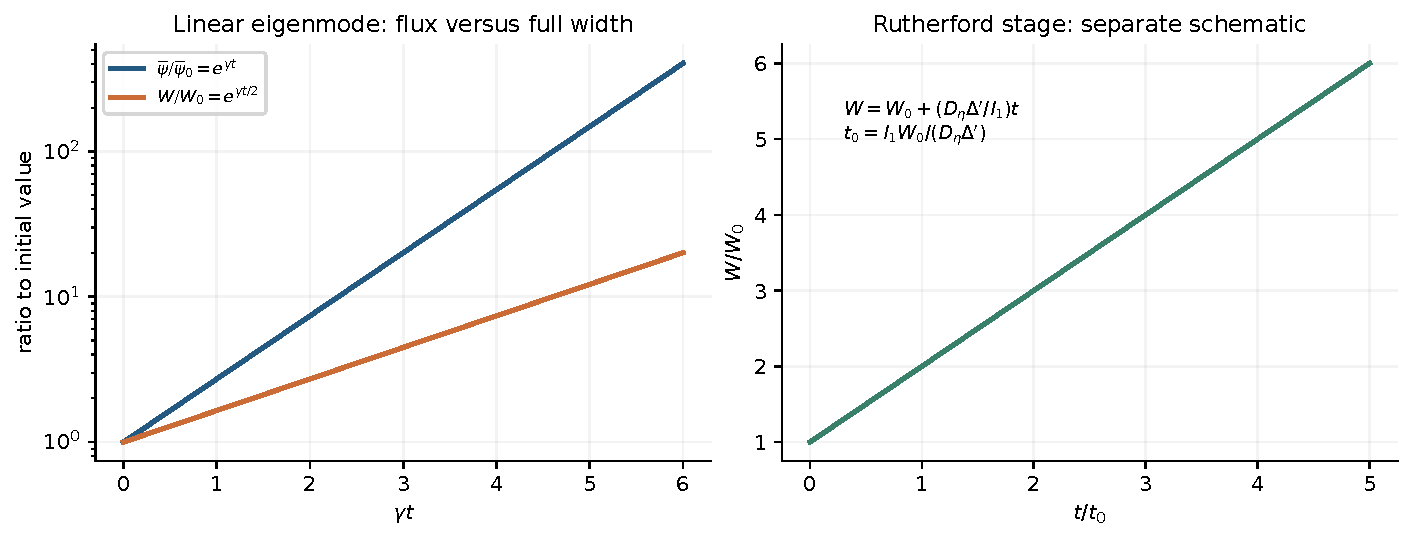
\includegraphics[width=\textwidth]{figures/tm_growth_observables.pdf}
\caption{不同观测量的增长曲线：在线性阶段，磁通幅和岛宽的半对数斜率分别为$\gamma$与$\gamma/2$。独立面板展示常$\Delta'$下Rutherford岛宽线性增长。各面板为解析教学曲线，没有强行拼成一条完整非线性时间轨道，也不是实验数据。}
\label{tm:fig:time}
\end{figure}

\section{一条长电流片为什么可能长出很多岛}
前面$a$是固定平衡片半厚。现在考虑长度尺度为$L$、厚度由Sweet--Parker平衡给出的长薄片。令
\begin{equation}
 S_L=\frac{LV_A}{D_\eta},\qquad \frac aL\sim S_L^{-1/2}.
\end{equation}
这里$L$的半长/全长约定会影响系数，本节只推导幂指数。最重要的一步是把\emph{局地片厚归一化}与\emph{全局长度归一化}分开：
\begin{equation}
 S_a=\frac{aV_A}{D_\eta}=\frac aL S_L\sim S_L^{1/2},
 \qquad \frac{\tau_{A,L}}{\tau_{A,a}}=\frac La\sim S_L^{1/2}.
\end{equation}
将式\eqref{tm:fastest}逐项换单位：
\begin{align}
 \gamma_{\max}\tau_{A,L}
 &=\left(\gamma_{\max}\tau_{A,a}\right)\frac La
 \sim S_a^{-1/2}S_L^{1/2}
 \sim\boxed{S_L^{1/4}},\label{tm:plasmoidgamma}\\
 k_{\max}L&=(k_{\max}a)\frac La
 \sim S_a^{-1/4}S_L^{1/2}
 \sim\boxed{S_L^{3/8}},\label{tm:plasmoidk}\\
 \frac{\delta_{\rm in}}L&=\frac{\delta_{\rm in}}a\frac aL
 \sim S_a^{-1/4}S_L^{-1/2}
 \sim\boxed{S_L^{-5/8}}.\label{tm:plasmoidwidth}
\end{align}
局地$\gamma\tau_{A,a}\sim S_L^{-1/4}\ll1$，却有全局$\gamma\tau_{A,L}\sim S_L^{1/4}\gg1$。两者不矛盾：厚度$a$远小于长度$L$，对应的Alfv\'en时间不同。所谓快于全局Alfv\'en时间，不意味着信号在局地超过光速或立即跨越整个系统。

以上重新获得plasmoid不稳定性的核心标度。Loureiro等的原始分析进一步采用带出流的薄片平衡并检查相应排序；这里的Harris式推导用于说明标度机制，不冒充与其平衡完全一致的数值系数。\citep{TMLoureiro2007}

\paragraph{再算一组长度、时间与岛数。}
取自设$L=10\,\mathrm m$、$V_A=10^5\,\mathrm{m/s}$、$D_\eta=0.01\,\mathrm{m^2/s}$，则$S_L=10^8$，
\begin{align}
 a&\sim10\times10^{-4}=1.0\,\mathrm{mm},&
 S_a&\sim10^4,\\
 \tau_{A,L}&=10^{-4}\,\mathrm s,&
 \gamma_{\max}&\sim10^2/\tau_{A,L}=10^6\,\mathrm{s^{-1}},\\
 \delta_{\rm in}&\sim10(10^8)^{-5/8}=10^{-4}\,\mathrm m,&
 k_{\max}L&\sim(10^8)^{3/8}=10^3.
\end{align}
因此局地增长时间约$1\,\mu\mathrm s$，内层约$0.1$毫米。若为长度$L$的周期示意区间，几何可容纳的波周期数约$k_{\max}L/(2\pi)\sim159$；开放出流片的最终可见岛数还会受排出、并合、噪声和非线性影响，不能把159当作实验应该拍到的精确岛数。

还必须检查出流。若出流率$V_A/L$与$\gamma$同阶或更大，小扰动可能在长成明显磁岛前已被排走；静态无限长片的本征增长率不能直接等同于有限寿命片的破碎时刻。经常出现的临界$S$量级也依赖噪声、边界、黏性和片形成历史，不是由式\eqref{tm:plasmoidgamma}单独推出的普适整数。

\section{电流片逐渐变薄：并不一定先形成稳态Sweet--Parker片}
设形成中的片有$a/L\sim S_L^{-\alpha}$。局地$S_a\sim S_L^{1-\alpha}$，因此
\begin{equation}
 \gamma_{\max}\tau_{A,L}
 \sim S_a^{-1/2}\frac La
 \sim S_L^{-(1-\alpha)/2+\alpha}
 =S_L^{(3\alpha-1)/2}.
\end{equation}
取$\alpha=1/3$可得到$\gamma_{\max}\tau_{A,L}\sim O(1)$。这是常被称为“理想撕裂”厚度标度的简单来源；名称指\emph{全局增长时间趋于Alfv\'en量级}，并不意味着内层变成严格理想、完全没有磁冻结破坏机制。若真的令所有非理想项为零且要求光滑解，不能借这个名称让磁力线凭空改变拓扑。

这个算式仍是假定背景片形状可用准静态序列描述。真正何时破碎还要比较片变薄率、种子谱与累计放大
\begin{equation}
 \ln\frac{\widetilde\psi(t)}{\widetilde\psi(t_0)}
 =\int_{t_0}^{t}\gamma[a(t'),k,\ldots]\,\dd t'.
\end{equation}
瞬时$\gamma$很大不等于已经积累足够增长；反之，较小增长率也可在长时间后产生显著磁岛。这里不代替完整动态形成理论。

\section{经典电阻理论何时需要交给双流体或动理学}
经典FKR推导中流体具有共同速度，并用$\eta\J$破坏磁冻结。真实电子--离子等离子体的欧姆律还可能包含
\begin{equation}
 \E+\vct u_i\times\B
 =\frac{\J\times\B}{en}
 -\frac{\nabla\cdot\vct P_e}{en}
 -\frac{m_e}{e}\left(\partial_t+\vct u_e\cdot\nabla\right)\vct u_e
 +\eta\J,\qquad
 \vct u_e=\vct u_i-\frac{\J}{en}.
\end{equation}
这里$n$为准中性数密度，$e>0$，$\vct P_e$为电子压力张量。它们各自需要不同变量与闭合。加入Hall项后磁场可相对离子运动，电子惯性和压力张量又改变更内层的平衡；不能只把FKR公式里的$\eta$换成一个“有效Hall电阻”。

常见微观长度为
\begin{equation}
 d_i=\sqrt{\frac{m_i}{\mu_0ne^2}},\quad
 d_e=\sqrt{\frac{m_e}{\mu_0ne^2}},\quad
 \rho_s=\frac{\sqrt{eT_e/m_i}}{\Omega_{ci}},\quad
 \Omega_{ci}=\frac{eB}{m_i}.
\end{equation}
此式$T_e$以eV表示，所以$eT_e$具有能量单位。$d_i$与离子--电子漂移尺度相关；强导场中的$\rho_s$、压力和声响应也可能进入排序。实际阈值应来自线性化后的各项比较，而不是任取一个长度就宣布所有情况下的转变点。\citep{TMHall2011}

\paragraph{把前面的数学算例放进真实参数会发生什么。}
以氢离子、$n=10^{20}\,\mathrm{m^{-3}}$计算，取$m_i=1.673\times10^{-27}\,\mathrm{kg}$、$e=1.602\times10^{-19}\,\mathrm C$，得到
\begin{align}
 d_i&=\sqrt{\frac{1.673\times10^{-27}}
 {(1.2566\times10^{-6})(10^{20})(1.602\times10^{-19})^2}}
 =2.28\times10^{-2}\,\mathrm m,\\
 d_e&=d_i\sqrt{m_e/m_i}=5.31\times10^{-4}\,\mathrm m.
\end{align}
第\ref{tm:matching}章算例的$\delta_*=5.63\times10^{-4}\,\mathrm m$于是满足
\begin{equation}
 d_i/\delta_*=40.5,\qquad d_e/\delta_*=0.94.
\end{equation}
这些长度比是重新检查双流体排序的警报，不能单独证明每一个电子惯性项都占主导。尤其是电子速度含$-\J/(en)$，其时间导数给广义欧姆定律带来的电流惯性项约为
\begin{equation}
 E_{\text{电子时间惯性}}
 \sim\frac{m_e}{ne^2}\gamma J
 =\mu_0d_e^2\gamma J.
\end{equation}
与电阻项$E_\eta=\eta J=\mu_0D_\eta J$比较，得到
\begin{equation}
 \frac{E_{\text{电子时间惯性}}}{E_\eta}
 \sim\frac{\gamma d_e^2}{D_\eta}
 =\frac{(250.97)(5.3146\times10^{-4})^2}{0.01}
 =7.09\times10^{-3}.
\end{equation}
所以即使$d_e/\delta_*\simeq0.94$，在这组增长率下，电子时间惯性仍只有电阻项的约$0.7\%$。原因是常磁通层内$\Psi''\sim\Delta'\Psi/\delta_*$，并非$\Psi/\delta_*^2$；仅按长度替换导数会丢失这个排序。上述比较只检查电子时间惯性，未检查电子对流惯性、压力及Hall耦合。较大的$d_i/\delta_*$仍提示必须把Hall响应代回线性方程比较，不能据经典FKR的内部排序就宣布它适用于这组实际等离子体。

若依然指定$V_A=10^5\,\mathrm{m/s}$，相应重联场为
$B_0=V_A\sqrt{\mu_0m_in}=0.0458\,\mathrm T$；它不会改变上述$d_i,d_e$。这正是要同时查长度、时间和各项实际幅值的原因。

此外需检查碰撞：局地电阻与流体热闭合通常要求相关时间和空间尺度上有足够的碰撞松弛。$\nu_{ei}\gg\gamma$是必要比较之一，却不能代替平行平均自由程$\lambda_{\rm mfp}$与实际梯度长度的比较。薄层里的$k_\parallel$接近共振而沿场连接长度很长，不能简单用$\delta$替代所有方向的梯度尺度。若压力张量、热流或粒子共振重要，应回到双流体矩方程或动理学方程，而不是对经典公式作无依据外推。

\section{与托卡马克撕裂模的桥梁：先认出共振条件}
在大长径比圆柱近似中，令$r,\theta,\zeta$分别为径向、极向和环向角，主半径为$R$。扰动相位写成$m\theta-n\zeta$，平衡场有$B_\theta,B_\zeta$。沿场导数作用于扰动给
\begin{equation}
 \B_0\cdot\nabla e^{i(m\theta-n\zeta)}
 =i\left(\frac{mB_\theta}{r}-\frac{nB_\zeta}{R}\right)
 e^{i(m\theta-n\zeta)}.
\end{equation}
定义安全因子$q(r)=rB_\zeta/(RB_\theta)$，括号可写为
\begin{equation}
 \frac{B_\theta}{r}[m-nq(r)].
\end{equation}
因此共振面满足$q(r_s)=m/n$。例如$2/1$模的共振面在$q=2$处；这与slab的$\vct k\cdot\B_0=0$是同一个逻辑。$q'(r_s)$决定局地磁剪切，与slab的$B'_0$相联系。

但圆柱/环形的外区方程、壁面响应和压力曲率不同，不能把Harris片$\Delta'$原封不动搬进托卡马克。新经典撕裂模还涉及磁岛内压强展平引起的bootstrap电流缺失及有限种子阈值；它可以在经典$\Delta'<0$时受到驱动。实验章将把这些结果与本章经典Rutherford方程分别对照，避免把所有“有磁岛”的信号都叫作同一个FKR验证。

\section{把整条推导链用自己的话串起来}
平衡磁场和电流给出自由能与磁剪切；边界和平衡共同决定外区解及$\Delta'$。共振面附近，理想冻结关系要求的流动奇异，迫使电阻与惯性进入一个很薄的层。层内电流的积分必须补上外区斜率差，这个匹配条件选择$\gamma$和$\delta$。常磁通与大$\Delta'$采用不同二阶导数量级，因此给出不同指数。磁岛宽度超过线性层后，非线性改变平流与电流分布；弱驱动小岛可进入磁面近似平衡的Rutherford增长。片若足够细长，会有许多沿片波长同时增长；继续变薄后又可能进入双流体或动理学尺度。

这条链中的每一箭头都有假设。真正掌握理论，意味着面对新参数时能够列出这些假设、算出各项比值、发现哪一步先失效，并据此选择新的方程；不是只会背诵一个$\eta^{3/5}$。
